
\section{Batterien und Akkus}
\label{section:batterien_und_akkus}
\begin{frame}%STARTCONTENT

\begin{columns}
    \begin{column}{0.48\textwidth}
    \begin{itemize}
  \item Spannung durch Ladungstrennung in elektrochemischen Vorgängen
  \item Beim Akku ist der Vorgang umkehrbar
  \item Plus- oder Minuspol gekennzeichnet
  \end{itemize}

    \end{column}
   \begin{column}{0.48\textwidth}
       
\begin{figure}
    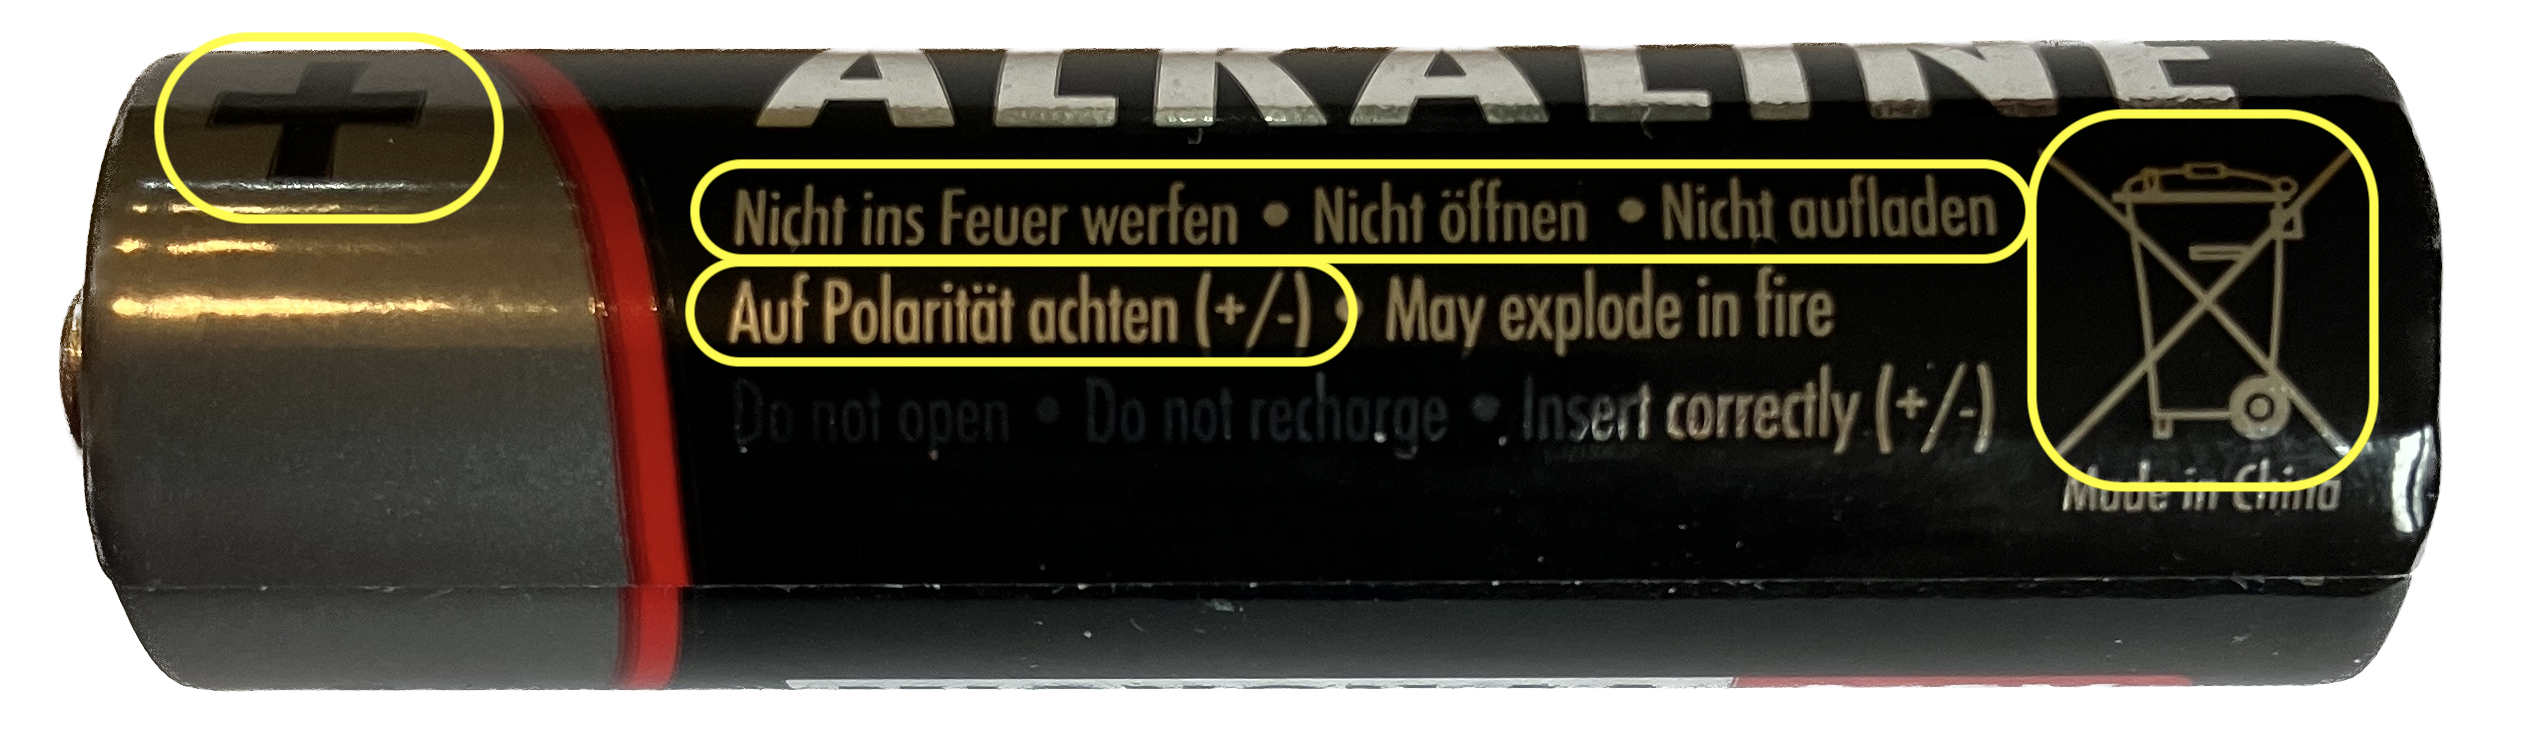
\includegraphics[width=0.85\textwidth]{foto/89}
    \caption{\scriptsize Eine Batterie mit Kennzeichnung der Pole und Warnhinweisen}
    \label{n_Bat_AA}
\end{figure}

\begin{figure}
    \DARCimage{0.85\linewidth}{517include}
    \caption{\scriptsize Schaltzeichen einer Batterie}
    \label{n_schaltzeichen_batt}
\end{figure}


   \end{column}
\end{columns}

\end{frame}

\begin{frame}
\only<1>{
\begin{PQuestion}{NB201}{Welches Bauteil wird durch das Schaltzeichen symbolisiert?}{Batterie}
{Diode}
{Widerstand}
{Kondensator}
{\DARCimage{0.5\linewidth}{510include}}\end{PQuestion}

}
\only<2>{
\begin{PQuestion}{NB201}{Welches Bauteil wird durch das Schaltzeichen symbolisiert?}{\textbf{\textcolor{DARCgreen}{Batterie}}}
{Diode}
{Widerstand}
{Kondensator}
{\DARCimage{0.5\linewidth}{510include}}\end{PQuestion}

}
\end{frame}

\begin{frame}
\only<1>{
\begin{PQuestion}{NB203}{Wie lauten die Bezeichnungen für die Anschlüsse 1 und 2 im Schaltsymbol?}{1 = Nord-Pol; 2 = Süd-Pol}
{1 = Minus-Pol; 2 = Plus-Pol}
{1 = Plus-Pol; 2 = Minus-Pol}
{1 = Süd-Pol; 2 = Nord-Pol}
{\DARCimage{0.5\linewidth}{517include}}\end{PQuestion}

}
\only<2>{
\begin{PQuestion}{NB203}{Wie lauten die Bezeichnungen für die Anschlüsse 1 und 2 im Schaltsymbol?}{1 = Nord-Pol; 2 = Süd-Pol}
{1 = Minus-Pol; 2 = Plus-Pol}
{\textbf{\textcolor{DARCgreen}{1 = Plus-Pol; 2 = Minus-Pol}}}
{1 = Süd-Pol; 2 = Nord-Pol}
{\DARCimage{0.5\linewidth}{517include}}\end{PQuestion}

}
\end{frame}

\begin{frame}
\frametitle{Serienschaltung}
\begin{columns}
    \begin{column}{0.48\textwidth}
    \begin{itemize}
  \item Batterien lassen sich hintereinander schalten
  \item Pluspol auf Minuspol der vorhergehenden Batterie
  \item Die Gesamtspannung ist die Summe der Einzelspannungen
  \end{itemize}

    \end{column}
   \begin{column}{0.48\textwidth}
       
\begin{figure}
    \DARCimage{0.85\linewidth}{748include}
    \caption{\scriptsize Verschiedene Batterien und Akkus}
    \label{batterien_und_akkus_sammlung}
\end{figure}


   \end{column}
\end{columns}

\end{frame}

\begin{frame}
\only<1>{
\begin{PQuestion}{NB204}{Folgende Schaltung besteht aus Spannungsquellen von je \qty{1,5}{\V}. Welche Spannung misst man zwischen den Kontakten, die mit \glqq +\grqq{} und \glqq -\grqq{} gekennzeichnet sind?}{\qty{0,25}{\V}}
{\qty{1,5}{\V}}
{\qty{9}{\V}}
{\qty{6}{\V}}
{\DARCimage{1.0\linewidth}{431include}}\end{PQuestion}

}
\only<2>{
\begin{PQuestion}{NB204}{Folgende Schaltung besteht aus Spannungsquellen von je \qty{1,5}{\V}. Welche Spannung misst man zwischen den Kontakten, die mit \glqq +\grqq{} und \glqq -\grqq{} gekennzeichnet sind?}{\qty{0,25}{\V}}
{\qty{1,5}{\V}}
{\textbf{\textcolor{DARCgreen}{\qty{9}{\V}}}}
{\qty{6}{\V}}
{\DARCimage{1.0\linewidth}{431include}}\end{PQuestion}

}
\end{frame}

\begin{frame}
\frametitle{Kurzschluss}
\begin{itemize}
  \item Vermeiden!
  \item Bei Akkus Gefahr der Überhitzung
  \item Brandgefahr
  \end{itemize}
\end{frame}

\begin{frame}
\only<1>{
\begin{QQuestion}{ND110}{Was ist bei der Verwendung von Akkus und Batterien zu beachten?}{Sie müssen paarweise verwendet werden.}
{Ein Kurzschluss ist zu vermeiden.}
{Sie müssen mit einem Mindestentladestrom betrieben werden.}
{Sie sollen stets vollkommen entladen werden.}
\end{QQuestion}

}
\only<2>{
\begin{QQuestion}{ND110}{Was ist bei der Verwendung von Akkus und Batterien zu beachten?}{Sie müssen paarweise verwendet werden.}
{\textbf{\textcolor{DARCgreen}{Ein Kurzschluss ist zu vermeiden.}}}
{Sie müssen mit einem Mindestentladestrom betrieben werden.}
{Sie sollen stets vollkommen entladen werden.}
\end{QQuestion}

}
 \end{frame}

\begin{frame}
\frametitle{Unsachgemäßer Umgang}
\begin{itemize}
  \item In Akkus sind verschiedene chemische Technologien im Einsatz
  \item Beim Aufladen angepasste Ladegeräte verwenden
  \item Gefahr von Überhitzung, Explosion oder Brand
  \item Dadurch kann es zu Verbrennungen, Verätzungen und Vergiftungen kommen
  \end{itemize}
\end{frame}

\begin{frame}
\only<1>{
\begin{QQuestion}{NK306}{Welche Gefahren drohen dem Anwender bei unsachgemäßem Umgang mit wiederaufladbaren Batterien?}{Verätzungen, Spannungsschwankungen, Ruhestromanstieg}
{Überstrom, Unterspannung, Leistungsreduzierung}
{Verbrennungen, Verätzungen, Vergiftungen}
{Anstieg des Innenwiderstands, Spannungsschwankungen, Leistungsreduzierung}
\end{QQuestion}

}
\only<2>{
\begin{QQuestion}{NK306}{Welche Gefahren drohen dem Anwender bei unsachgemäßem Umgang mit wiederaufladbaren Batterien?}{Verätzungen, Spannungsschwankungen, Ruhestromanstieg}
{Überstrom, Unterspannung, Leistungsreduzierung}
{\textbf{\textcolor{DARCgreen}{Verbrennungen, Verätzungen, Vergiftungen}}}
{Anstieg des Innenwiderstands, Spannungsschwankungen, Leistungsreduzierung}
\end{QQuestion}

}
 \end{frame}%ENDCONTENT
